\documentclass[varwidth=true, border=2pt]{standalone}
\usepackage{pgfplots}
\pgfplotsset{compat=1.18}
\usepackage{xcolor}

\begin{document}

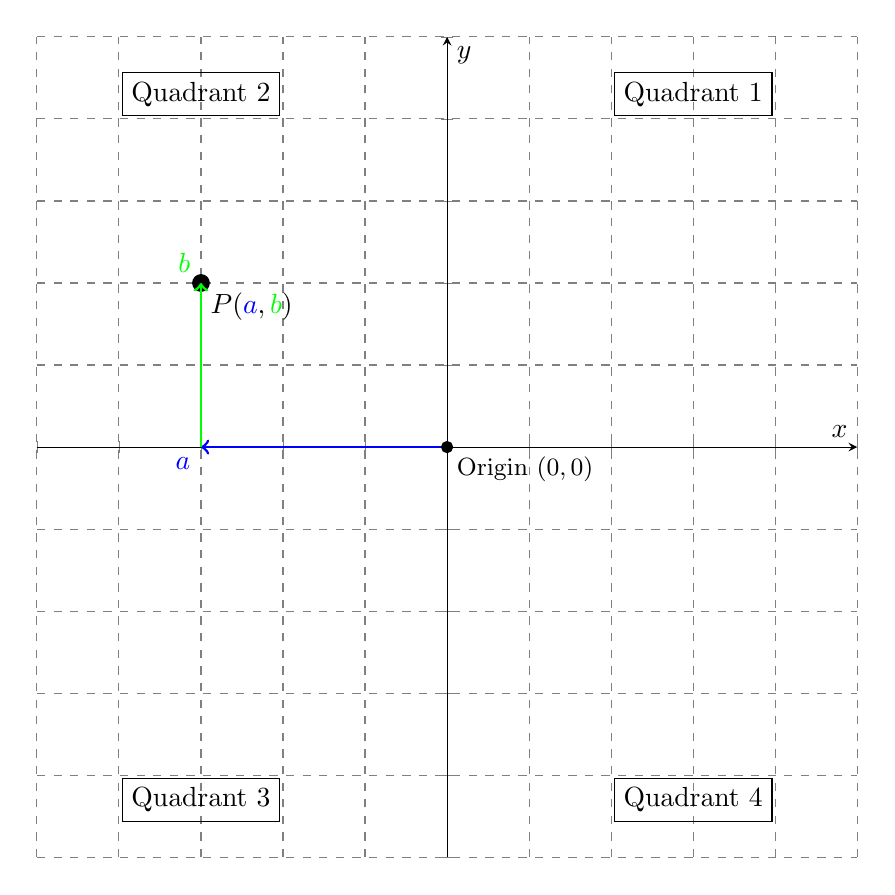
\begin{tikzpicture}
	\begin{axis}[
			xmin=-5, xmax=5,
			ymin=-5, ymax=5,
			axis lines=middle,
			xlabel=$x$,
			ylabel=$y$,
			grid=major,
			grid style={dashed, gray},
			xtick={-5,-4,-3,-2,-1,0,1,2,3,4,5},
			ytick={-5,-4,-3,-2,-1,0,1,2,3,4,5},
			xticklabels={},
			yticklabels={},
			width=12cm, height=12cm
		]
		% Point P
		\filldraw (-3,2) circle (3pt)
		node[anchor=north west] {$P(\textcolor{blue}{a}, \textcolor{green}{b})$};

		% Horizontal arrow
		\draw[->, blue, line width=1pt] (0,0) -- (-3,0)
		node[anchor=north east] {$a$};

		% Vertical arrow
		\draw[->, green, line width=1pt] (-3,0) -- (-3,2)
		node[anchor=south east] {$b$};

		% Origin
		\filldraw (0,0) circle (2pt)
		node[anchor=north west] {\small Origin $(0, 0)$};

		% Quadrant labels
		\node[draw] at (3, 4.3) {Quadrant 1};
		\node[draw] at (-3, 4.3) {Quadrant 2};
		\node[draw] at (-3, -4.3) {Quadrant 3};
		\node[draw] at (3, -4.3) {Quadrant 4};
	\end{axis}
\end{tikzpicture}

\end{document}
